\documentclass{extarticle}
\sloppy

%%%%%%%%%%%%%%%%%%%%%%%%%%%%%%%%%%%%%%%%%%%%%%%%%%%%%%%%%%%%%%%%%%%%%%
% PACKAGES            																						  %
%%%%%%%%%%%%%%%%%%%%%%%%%%%%%%%%%%%%%%%%%%%%%%%%%%%%%%%%%%%%%%%%%%%%%
\usepackage[10pt]{extsizes}
\usepackage{amsfonts}
\usepackage{amsthm}
\usepackage{amssymb}
\usepackage[shortlabels]{enumitem}
\usepackage{microtype} 
\usepackage{amsmath}
\usepackage{mathtools}
\usepackage{commath}
\usepackage[margin=1in]{geometry}
\usepackage{float}
\usepackage{cancel}
\usepackage{amsmath, amsfonts, amssymb}

%%%%%%%%%%%%%%%%%%%%%%%%%%%%%%%%%%%%%%%%%%%%%%%%%%%%%%%%%%%%%%%%%%%%%%
% PROBLEM ENVIRONMENT         																			           %
%%%%%%%%%%%%%%%%%%%%%%%%%%%%%%%%%%%%%%%%%%%%%%%%%%%%%%%%%%%%%%%%%%%%%
\usepackage{tcolorbox}
\tcbuselibrary{theorems, breakable, skins}
\newtcbtheorem{prob}% environment name
              {Problem}% Title text
  {enhanced, % tcolorbox styles
  attach boxed title to top left={xshift = 4mm, yshift=-2mm},
  colback=blue!5, colframe=black, colbacktitle=blue!3, coltitle=black,
  boxed title style={size=small,colframe=gray},
  fonttitle=\bfseries,
  separator sign none
  }%
  {} 
\newenvironment{problem}[1]{\begin{prob*}{#1}{}}{\end{prob*}}

%%%%%%%%%%%%%%%%%%%%%%%%%%%%%%%%%%%%%%%%%%%%%%%%%%%%%%%%%%%%%%%%%%%%%%
% THEOREMS/LEMMAS/ETC.         																			  %
%%%%%%%%%%%%%%%%%%%%%%%%%%%%%%%%%%%%%%%%%%%%%%%%%%%%%%%%%%%%%%%%%%%%%%
\newtheorem{thm}{Theorem}
\newtheorem*{thm-non}{Theorem}
\newtheorem{lemma}[thm]{Lemma}
\newtheorem{corollary}[thm]{Corollary}

%%%%%%%%%%%%%%%%%%%%%%%%%%%%%%%%%%%%%%%%%%%%%%%%%%%%%%%%%%%%%%%%%%%%%%
% MY COMMANDS   																						  %
%%%%%%%%%%%%%%%%%%%%%%%%%%%%%%%%%%%%%%%%%%%%%%%%%%%%%%%%%%%%%%%%%%%%%
\newcommand{\Z}{\mathbb{Z}}
\newcommand{\R}{\mathbb{R}}
\newcommand{\C}{\mathbb{C}}
\newcommand{\F}{\mathbb{F}}
\newcommand{\bigO}{\mathcal{O}}
\newcommand{\Real}{\mathcal{Re}}
\newcommand{\poly}{\mathcal{P}}
\newcommand{\mat}{\mathcal{M}}
\DeclareMathOperator{\Span}{span}
\newcommand{\Hom}{\mathcal{L}}
\DeclareMathOperator{\Null}{null}
\DeclareMathOperator{\Range}{range}
\newcommand{\defeq}{\vcentcolon=}
\newcommand{\restr}[1]{|_{#1}}


%%%%%%%%%%%%%%%%%%%%%%%%%%%%%%%%%%%%%%%%%%%%%%%%%%%%%%%%%%%%%%%%%%%%%%
% SECTION NUMBERING																				           %
%%%%%%%%%%%%%%%%%%%%%%%%%%%%%%%%%%%%%%%%%%%%%%%%%%%%%%%%%%%%%%%%%%%%%%
\renewcommand\thesection{\Alph{section}:}
\renewcommand\thesubsection{\Alph{section}.\arabic{subsection}}
\renewcommand\thesubsubsection{\Alph{section}.\arabic{subsection}.\arabic{subsubsection}}


%%%%%%%%%%%%%%%%%%%%%%%%%%%%%%%%%%%%%%%%%%%%%%%%%%%%%%%%%%%%%%%%%%%%%%
% DOCUMENT START              																			           %
%%%%%%%%%%%%%%%%%%%%%%%%%%%%%%%%%%%%%%%%%%%%%%%%%%%%%%%%%%%%%%%%%%%%%%
\title{\vspace{-2em}Chapter 7: The Labor Market}
\author{\emph{Summary}, by JF Viray}
\date{}

\begin{document}
\maketitle

\section{Context on the Labor Market}
The labor force ($L$) consists of those who are working ($N$) or looking for work ($U$). The participation rate is equal to the ratio of the labor force to the working-age population. More importantly, the unemployment rate ($u$) is equal to the ratio of the number of unemployed to the number in the labor force, so
$$u = \frac{U}{L}$$

The US labor market is characterized by large flows between employment, unemployment, and “out of the labor force.”
On average, each month, about 44\% of the unemployed move out of unemployment, either to take a job or to drop out of the labor force. The opposite of this active labor market is called a scelerotic labor market with a stagnant unemployment pool. Let us now begin with how wages are actually determined. 
\section{Wage-Setting Relation}
\subsection{Bargaining Power}
Wages can be determined collectively, through unions, or individually. In the case of unions, this process is called collective bargaining. For individuals, bargaining power depends on how difficult it is to replace them and how costly retraining would be. Thus, there are two main ways to strengthen individual bargaining power
\begin{enumerate}
  \item Increase the skills needed to do your job; the more rare the skills, the harder it is to replace you.
  \item Bargain when the unemployment rate ($u$) is low since fewer job seekers make it harder for firms to find replacements. Conversely, when unemployment is high, firms can more easily replace workers. As a result, wages ($W$) are inversely related to the unemployment rate ($u$).
\end{enumerate}
\subsection{Efficiency Wages}

Firms avoid constant rehiring and retraining by paying wages above the reservation wage, making it more attractive for employees to stay. 
When the unemployment rate ($u$) is low, workers can easily find other jobs, so firms must offer higher wages to retain them. 
Conversely, when the unemployment rate is high, workers have fewer outside options, and firms can pay less. 
Similar to the Bargaining Power Theory, wages ($W$) are inversely related to the unemployment rate ($u$).

\subsection{Dealing with the two other variables of $P^e$ and $z$}
In both theories of how employees and firms set wages, workers must recognize that wages are determined in nominal (dollar) terms. 
Since the actual price level is not yet known during bargaining, they rely on their best estimate, the expected price level ($P^e$). As such, if the expected price were to increase, we should expect workers to bargain for higher wages.

Finally, we have a catch-all variable $z$ to represent other factors such as unemployment insurance and employment protection. Higher unemployment benefits increase the wage because workers now have higher bargaining power because firms don't want to pay the unemployment benefits. Similarly, an increase in employment protection increases the bargaining power of workers.

Wages are then modeled as a function on the expected price ($P^e$), wage ($W$), and other factors ($z$):
$$W = P^e F\underset{(-}{(u}\underset{, +)}{, z)} $$

\section{Price-Setting Relation}
Remember from our microeconomics course, the the marginal cost of production (the cost
of producing one more unit of output) is equal to the wage ($W$). In an ideal world of perfect competition, the price of a good ($P$) is the marginal cost of production, which is $W$, so $P = W$. However, firms are not always in a perfectly competitive market and can thus usually add a markup $m$. As such, the more realistic way of determining the prices of goods is:
$$P = (1+m) W$$.

\section{The Natural Rate of Unemployment ($u_n$)}
We shall now make a very BIG assumption to determine the natural rate of unemployment. We will suppose that \textbf{the actual price matches the expected price}, so $P = P^e$. This is reasonable in the medium run since the expected price eventually aligns to the actual price. This is why we call what we shall derive as the `natural' rate of unemployment. For the wage-setting relation, we will divide both sides by the actual price level $P$ to get the real wage $\frac{W}{P}$ to have:
$$W = P F\underset{(-}{(u}\underset{, +)}{, z)} \implies \frac{W}{P} = F\underset{(-}{(u}\underset{, +)}{, z)}$$
Let us also try to see how the real wage is determined based on Section C of Price Determination.
$$P = (1+m) W \implies \frac{P}{W} = 1+m \implies \frac{W}{P} = \frac{1}{1+m}$$
This suggest that as the markup ($m$) increases, the real wage ($\frac{W}{P}$) decreases. This makes sense since if we suppose that all the firms increase their markup, then all of the prices of goods become more expensive. In effect, your wage becomes weaker and thus the real wage decreases. 

Similar to what we did with the IS-LM model, let us now see the equilibrium that we get for the wage-setting and price-setting relations as shown in Figure 1. 
Equilibrium in the labor market requires that the real wage chosen in the wage-setting relation be equal to the real wage implied by the price-setting relation. As shown in the figure below of the labor market, this equilibrium point is at the natural rate of unemployment ($u_n$) where it is determined by $$F(u_n, z) = \frac{1}{1+m}$$

\begin{figure}[h]
    \centering 
    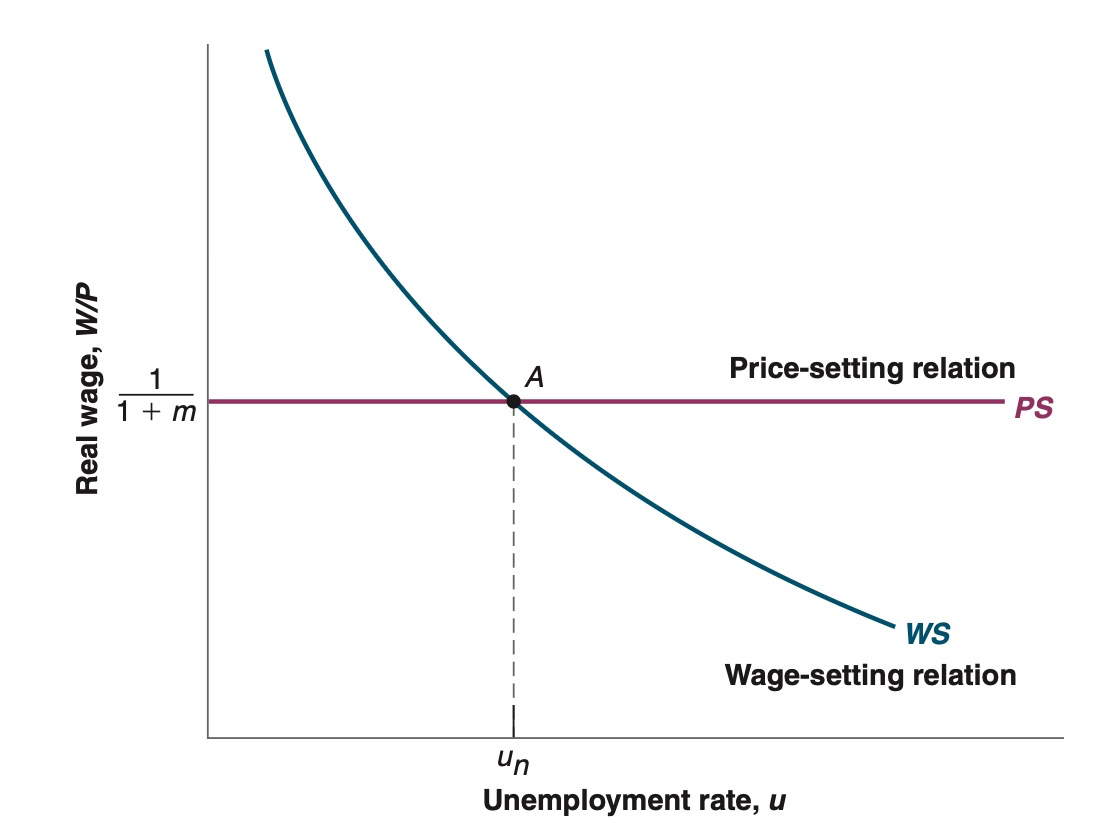
\includegraphics[width=0.3\linewidth]{labor market.png} 
    \caption{Equilibrium in the Labor Market} 
    \label{fig:derivation} 
\end{figure}

You can now start playing with the variables where you can ask what happens to the natural rate of unemployment $u_n$ if $z$ or $m$ increases? (Hint: If $z$ increases, the wage-setting relation has to shift upwards. If $m$ increases, the price-setting relation shifts downwards.)
\end{document}